\documentclass[letter,11pt]{article} % Tamaño de página y letra, tipo de documento
\usepackage[top = 2.0cm, bottom = 2.0cm, left = 2.0cm, right = 2.0cm]{geometry}

%% Comandos para codificación de archivo
\usepackage[utf8]{inputenc}
\usepackage[spanish,es-tabla]{babel}
\spanishdecimal{.}

%%%%%%%%%%%%%%%%%%%%%%%%%%%%%%%%%%%%%%%%%%%%%%%%
%% Bibliotecas útiles %%
\usepackage{multirow} % Múltiples renglones
\usepackage{multicol} % Múltiples columnas
\usepackage{booktabs} % Tablas más estéticas
\usepackage{graphicx} % Agregar figuras
\usepackage{setspace}  % Quita sangría de inicio de párrafos
\setlength{\parindent}{0in}
\usepackage{float} % Control de ubicación de figuras
\usepackage{fancyhdr} % Formato de encabezados
\usepackage{amsmath,mathtools,amsfonts,amssymb} % Símbolos matemáticos
\usepackage{xcolor} % Texto y ecuaciones en color
\usepackage{pdfpages} % Insertar PDFs
\usepackage{hyperref}
\newcommand{\Heaviside}{\mathrm{H}}
%%%%%%%%%%%%%%%%%%%%%%%%%%%%%%%%%%%%%%%%%%%%%%%%
%% Encabezado y pie de página %%
\pagestyle{fancy}  
\fancyhf{} 
%%%%%%%%%%%%%%%%%%%%%%%%%%%%%%%%%%%%%%%%%%%%%%%%
\lhead{\footnotesize Entorno y Herramientas de software | Tarea 01} 
\rhead{\footnotesize LIRA} 
\cfoot{\footnotesize \thepage} 
%%%%%%%%%%%%%%%%%%%%%%%%%%%%%%%%%%%%%%%%%%%%%%%%
%% Aquí comienza la edición del documento

\begin{document}
	\thispagestyle{empty} % Sin encabezado en la primera página
	
	%%%%%%%%%%%%%%%%%%%%%%%%%%%%%%%%%%%%%%%%%%%%%%%%
	%% Datos para la primera página
	\begin{tabular} {p{14cm} p{3cm}}
		&  \multirow{3.5}{*}{
\includegraphics[scale=0.35]{Imagenes/UNAM_logo}}\\
		{\large \bf Laboratorio de Innovación y Robótica Avanzada} & \\
		{\large \bf LIRA} & \\
		UNAM | FI & \\
		&  \\
		\hline
	\end{tabular} 
	
	\vspace*{0.3cm} 
	
	\begin{center}
		{\Large \bf Tarea 01} \\
		{\bf {\normalsize Entorno y Herramientas de software}} \\
		\vspace{2mm} 
	\end{center}
	
	%Documento
	
	\section{Requisitos Mínimos Recomendados de Hardware}
	
	\textbf{Hardware Mínimo:}
	
	\begin{itemize}
		\item \textbf{CPU:} Procesador de 4 núcleos (Intel i5 o AMD Ryzen 5)
		\item \textbf{RAM:} 8 GB en DDR4
		\item \textbf{GPU:} Tarjeta gráfica dedicada con 2 GB VRAM (NVIDIA GTX 1050 / Radeon R9 280X o superior)
	\end{itemize}
	
	\textbf{Hardware recomendado:}
	
	\begin{itemize}
		\item \textbf{CPU:} Procesador de 8 núcleos (Intel i7/i9 o AMD Ryzen 7/9)
		\item \textbf{RAM:} 16-32 GB en DDR4/DDR5
		\item \textbf{GPU:} Tarjeta gráfica dedicada con 4 o 8 GB VRAM (NVIDIA RTX 2060 / Radeon RX 5600 XT o superior)
	\end{itemize}
	
	\section{Sistema operativo}
	
	Se necesita tener un sistema operativo (S.O) basado en GNU/Linux específicamente Ubuntu 24.04 o Ubuntu 22.04, ya sea en Maquina Virtual o de forma nativa. \textbf{Se recomienda utilizar Ubuntu 24.04 ya que es el S.O de desarrollo.}\\
	
	
	En este documento se muestra el método de instalación para Ubuntu 24.04, tanto de Maquina Virtual o de forma nativa (\textbf{\textit{DualBoot}})
	
	\begin{enumerate}
		\item \textbf{Descarga de la ISO}
		
		Descarga la ISO de Ubuntu 24.04 LTS desde la página oficial. \url{https://releases.ubuntu.com/noble/}
		
		\begin{figure}[H]
			\centering
			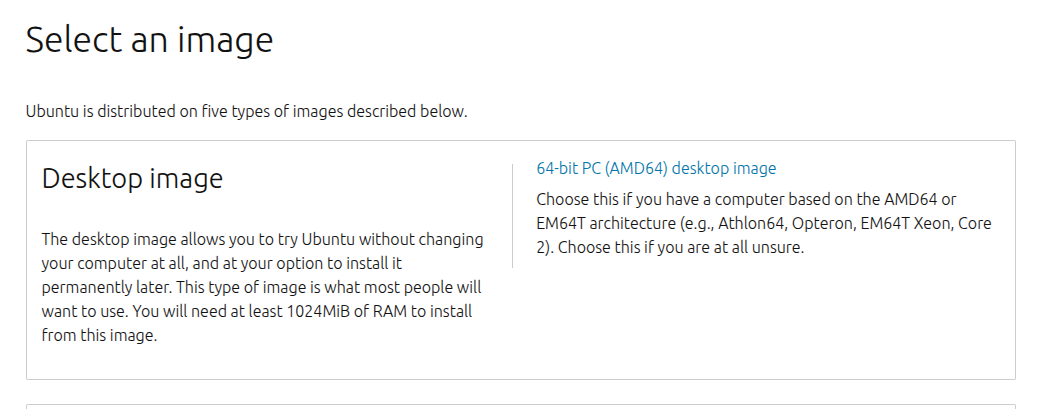
\includegraphics[width=0.5\linewidth]{Imagenes/ISO}
			\label{fig:iso}
		\end{figure}
		
		Seleccionar la opción de \textit{Desktop Image}.
		
		\item \textbf{Descarga y uso de la Maquina Virtual.}
		
		Si se opta por usar una Maquina Virtual (VM) se debe de descargar Oracle Virtual desde \url{https://www.virtualbox.org/} o cualquier otro Software virtualizador de su agrado como VMware de IBM.
		
		Una vez instalada, se debe de iniciar la aplicación (\textbf{\textcolor{red}{Nota:}} \textit{Si se esta en Windows se debe de activar la virtualización del CPU en la BIOS de tu dispositivo.})
		
		\begin{figure}[H]
			\centering
			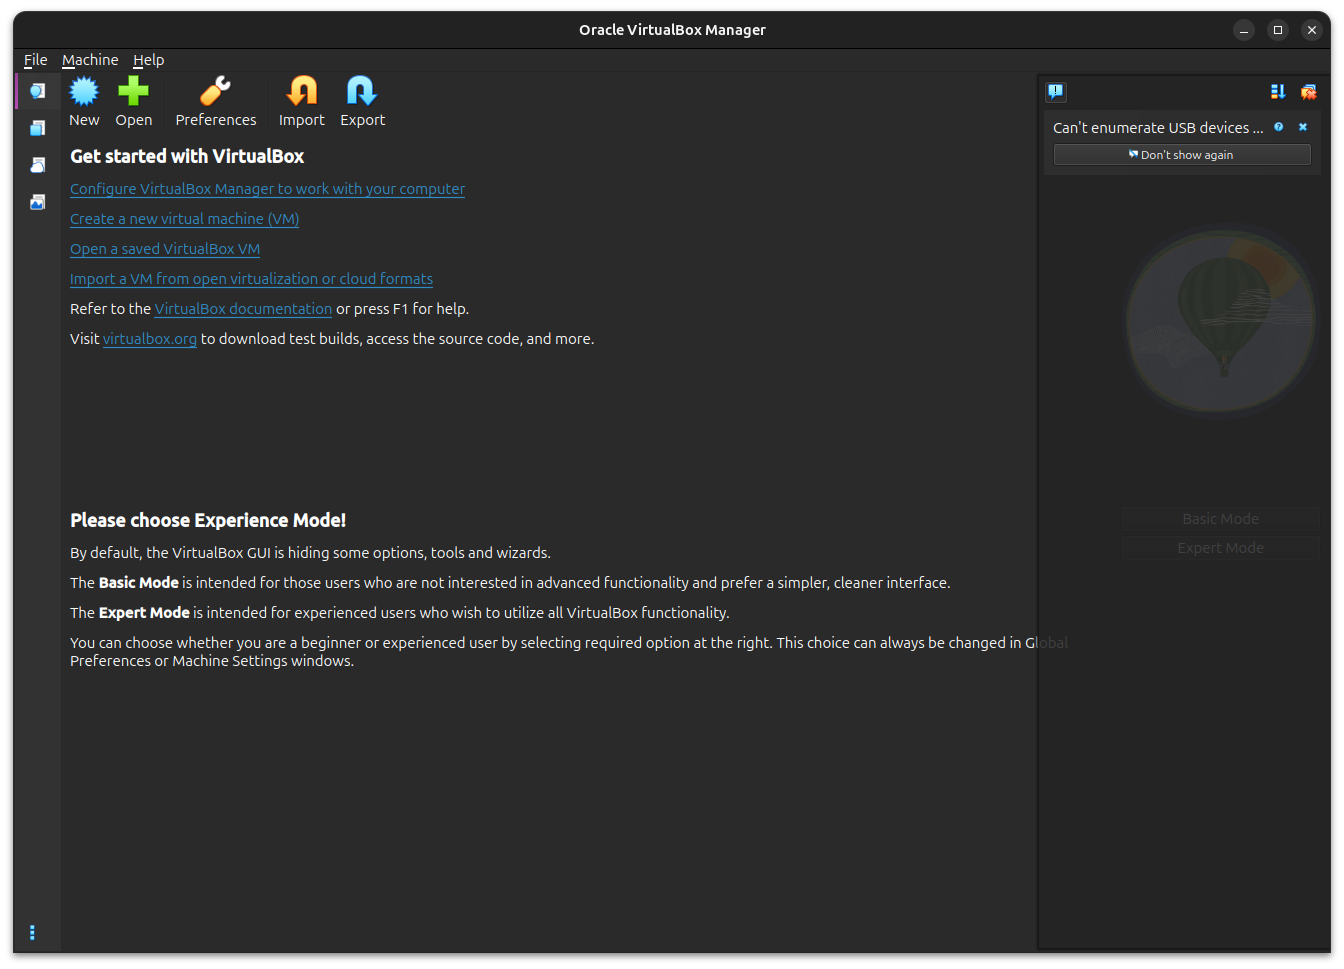
\includegraphics[width=0.4\linewidth]{Imagenes/Vm}
			\caption{Inicio de VirtualBox}
			\label{fig:vm}
		\end{figure}
		
		Una vez instalada e iniciada se agrega una nueva VM en \textit{"New"} y agregar las siguientes opciones:
		
		\begin{figure}[H]
			\centering
			\includegraphics[width=0.5\linewidth]{Imagenes/confiVM}
			\caption{Configuración inicial de la VM}
			\label{fig:confivm}
		\end{figure}
		
		Importante en la ruta para \textit{ISO Image} seleccionar la ISO descargada previamente mediante el directorio o explorador de archivos. Una vez seleccionada las demás parte se auto completaran así que no es necesario moverlas manualmente. Una vez hecho esto darle en \textbf{Next}.
		
		Una vez hecho esto se necesitará asignar los recursos que tendrá disponibles la VM creada, así como aparece en la imagen siguiente:
		
		\begin{figure}[H]
			\centering
			\includegraphics[width=0.5\linewidth]{Imagenes/Asignación}
			\caption{Asignación de recursos}
			\label{fig:asignacion}
		\end{figure}
		
		\textbf{¿Cómo se cuánto asignar?} \\
		La asignación de recursos dependerá de cada equipo de cómputo ya que no todos tienen las mismas características, es por eso que no existe un estándar como tal pero se puede seguí estas recomendaciones:
		
		\begin{itemize}
			\item \textbf{Asignación de RAM}
			\begin{itemize}
				\item Si el equipo cuenta con \textbf{4GB} o \textbf{menos}, se deberá de asignar  $\frac{3}{4}$ partes de la RAM.
				
				\item Si el equipo cuenta con \textbf{8GB} o \textbf{más}, se deberá asignar la mitad de memoria RAM.
			\end{itemize}
			
			
			\item \textbf{Asignación de CPU's o núcleos}
			\begin{itemize}
				\item Si se tiene en el equipo principal menos de \textbf{12} CPU's, asignar \textbf{4} núcleos.
				
				\item Si se tiene \textbf{12} o más asignar \textbf{6} o \textbf{8} CPU's
			\end{itemize}
			
			\item \textbf{Asignación de Disk Size}
			\begin{itemize}
				\item Si se cuenta con un espacio de \textbf{256 GB}, se deberá de asignar entre \textbf{30GB} y \textbf{50GB}
				
				\item Si se cuenta con 500GB, 1TB o más, se podrá asignar de \textbf{100GB} o más a elección del usuario.
			\end{itemize}
			
		\end{itemize}
		
		Para este último apartado en este caso como solo se trabajará para el simulador de este proyecto, se recomienda usar entre \textbf{30GB} y \textbf{50GB}. \\
		
		La siguiente ventana que saldrá es donde se deberá de asignar un nombre de usuario para esa VM y una contraseña, este paso es personal, aunque se recomienda que se ponga una contraseña \textbf{fácil} y \textbf{rápida} ya que se usará en varias ocasiones.
		
		\begin{figure}[H]
			\centering
			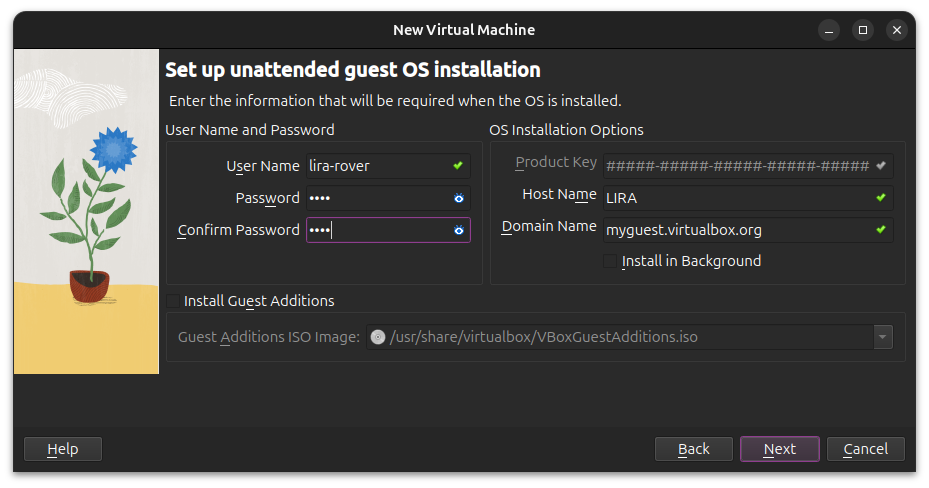
\includegraphics[width=0.5\linewidth]{Imagenes/username}
			\caption{Configuración de user name y password}
			\label{fig:username}
		\end{figure}
		
		Finalmente saldrá una ventana con la recopilación de los datos que se asignaron o definieron, se recomienda que se verifique cada una de la información que aparece, de esta manera si algo esta mal corregirlo a tiempo, una vez verificado se procede a darle en \textbf{Finish}. Una vez hecho esto comenzará a iniciar la ejecución de la maquina virtual.
		
		\item \textbf{Descarga de Ubuntu en DualBoot (nativo)}
		
		La otra opción y la recomendada es instalar Ubuntu de manera nativa en su equipo de cómputo, ya que de esta manera tendrá menos problemas de ejecución a la hora de hacer las pruebas ya que la asignación de recursos la hace con el 100\% de tu equipo mediante lo vaya requiriendo, como lo hace Windows o MacOS.\\
		
		Se tiene que tener en cuenta como consideración que para instalar el sistema operativo se requiere contar con un equipo de \textbf{64 bits} con al menos \textbf{4GB} de memoria RAM y mínimo \textbf{100GB} de espacio de almacenamiento libres.\\
		
		\textbf{\textcolor{red}{Nota Importante:}} Este proceso no genera daños en el equipo si se hace de manera correcta, a su vez se recomienda tener un respaldo de los documentos importantes de su computadora. Se aclara que el \textbf{DualBoot} hace que se pueda seguir ocupando tu sistema operativo de forma normal. Pero ahora con la opción de poder tener alguna de las siguientes combinaciones:
		
		\begin{itemize}
			\item Windows (8/10/11) y Ubuntu 24.04
			\item MacOS y Ubuntu 24.04
			\item Ubuntu 20.04 y Ubuntu 24.04 
		\end{itemize}
		
		Para iniciar con la instalación de Ubuntu 24.04 de forma nativa se necesita una USB de 8GB mínimo (aquí se guardará la ISO que previamente se descargo en el punto 1.) mediante un programa especial, a este proceso se le conoce como \textbf{USB Booteable o de arranque}. \\
		
		\textbf{En este manual de instalación se mostrará como se realiza en Windows como S.O principal y Ubuntu 24.04 como secundario}
		
		\textbf{\textcolor{red}{Nota:}} La USB usada para este proceso al necesitar un formato especifico ya no será capaz de guardar archivos comunes, y si es una usb que ya contiene archivos estos se perderán.\\
		
		Se tendrá que instalar el Software llamado \textbf{RUFUS} de su sitio oficial: \url{https://rufus.ie/es/}
		
		Una vez instalado e iniciado se procede a conectar la USB al equipo de cómputo, este programa despega una ventana en donde se pondrán las siguientes especificaciones:
		
		\begin{figure}[H]
			\centering
			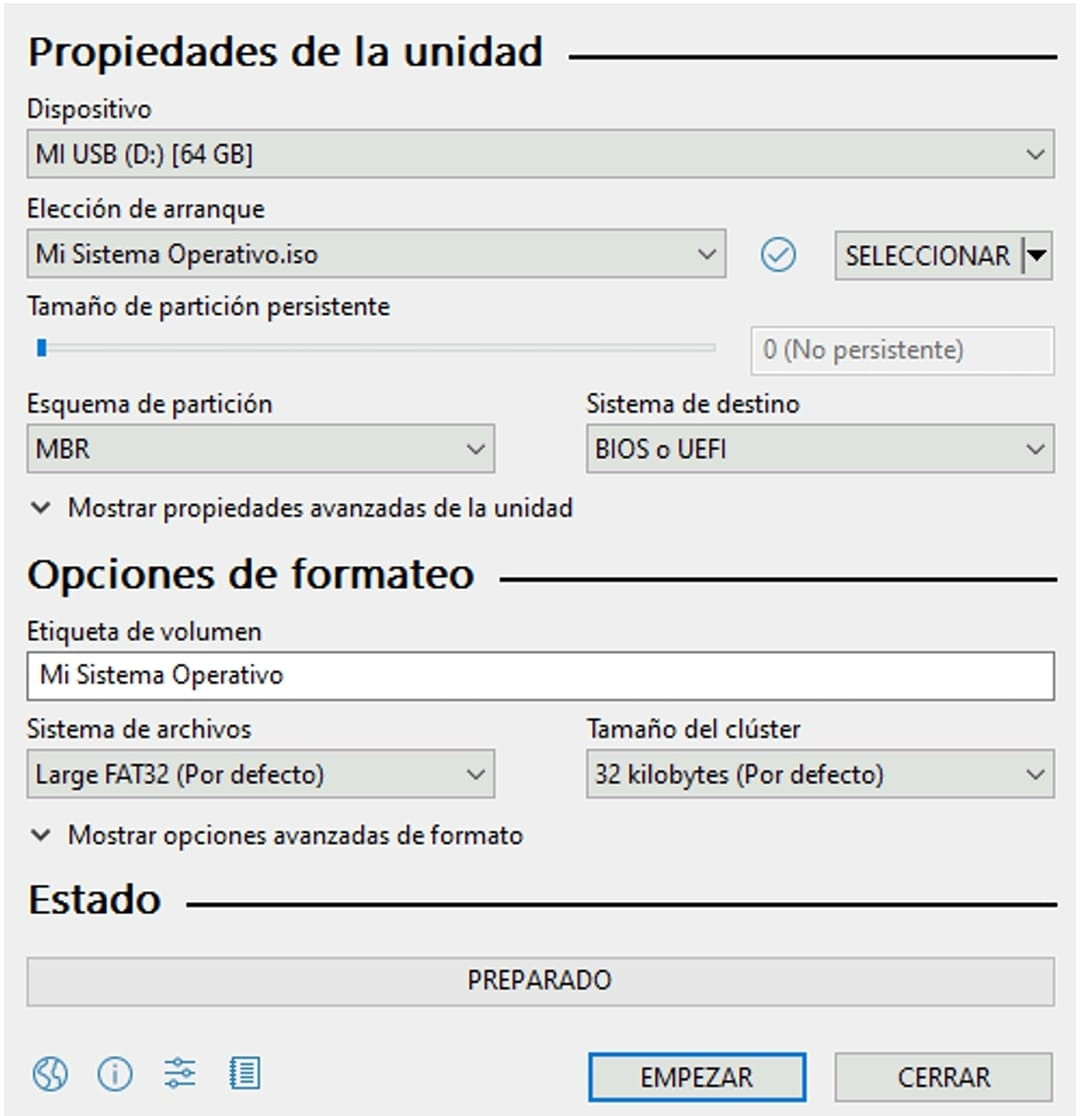
\includegraphics[width=0.5\linewidth]{Imagenes/rufus}
			\caption{Configuración de USB Booteable}
			\label{fig:rufus}
		\end{figure}
		
		Una vez puesto estas opciones, y seleccionar la dirección de la USB que se usará, darle en \textit{\textbf{Empezar}}, si es que sale la advertencia siguiente, se tendrá que seleccionar la opción \textit{\textbf{Escribir en modo Imagen ISO (recomendado)}}.
		
		\begin{figure}[H]
			\centering
			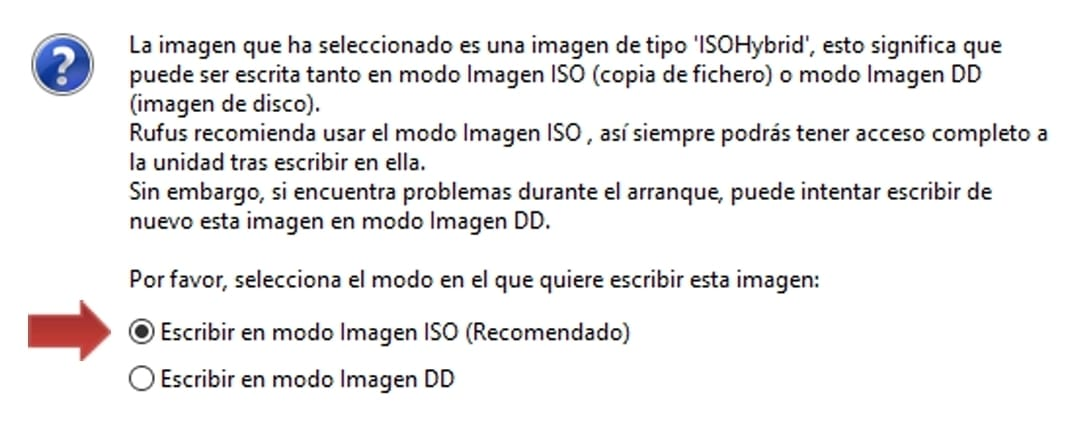
\includegraphics[width=0.5\linewidth]{Imagenes/advertencia}
			\caption{}
			\label{fig:advertencia}
		\end{figure}
		
		\textbf{En el caso de que salte una advertencia sobre el formateo total de la USB, aceptarlo.}
		
		\begin{figure}[H]
			\centering
			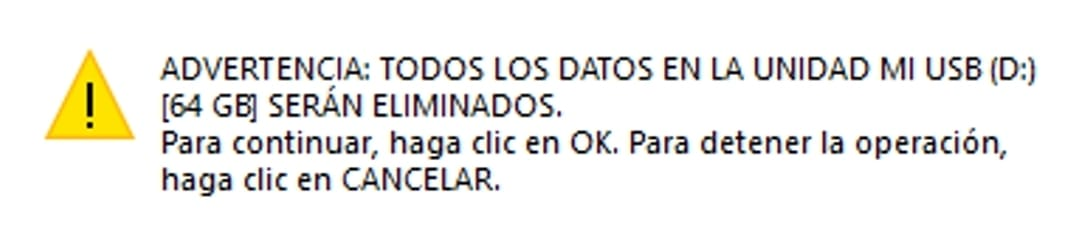
\includegraphics[width=0.5\linewidth]{Imagenes/adv_usb}
			\caption{Advertencia de USB}
			\label{fig:advusb}
		\end{figure}
		
		Una vez terminada la instalación se tendrá que revisar la información y archivos que contiene la USB, en este caso tendrán que aparecer algo parecido o idéntico a lo siguiente:
		
		\begin{figure}[H]
			\centering
			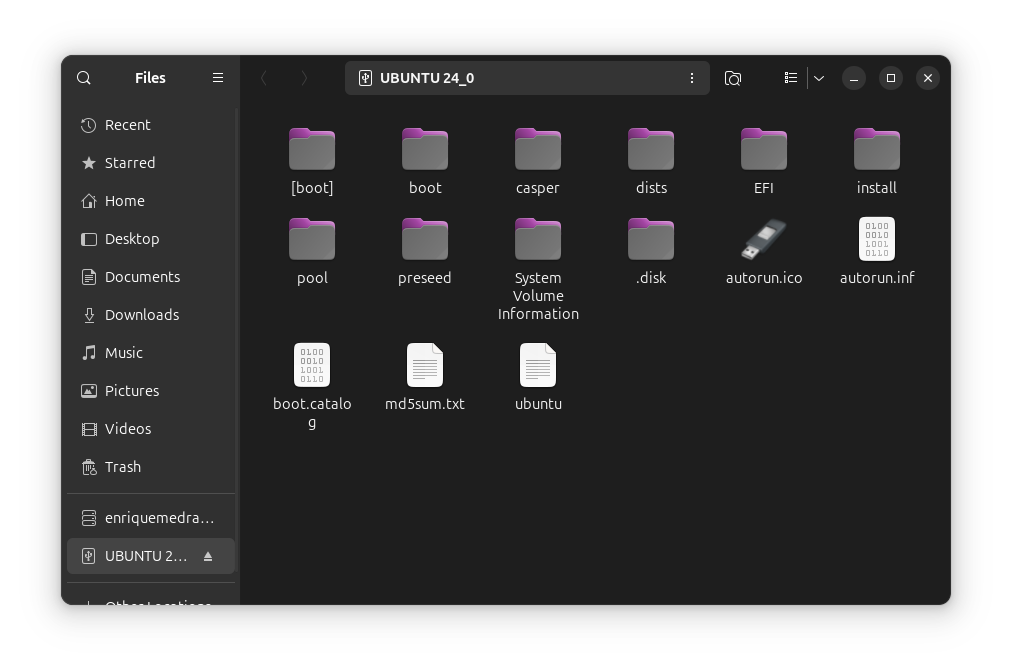
\includegraphics[width=0.5\linewidth]{Imagenes/carpeta_usb}
			\caption{Archivos dentro de la USB Booteable.}
			\label{fig:carpetausb}
		\end{figure}
		
		Ahora se tendrá que hacer la partición del Disco, esto permite asignar un espacio vacío de nuestra unidad de almacenamiento (Es aquí donde se instalará Ubuntu más adelante.), esto se hará desde un programa predeterminado de Windows como lo muestra el siguiente video: \url{https://youtu.be/fBgcoRKGprY?si=htWxP-L-xLJNoH2Q}.
		
		\textbf{\textcolor{red}{Nota:}} Solo crear una partición vacía (Tendrá que decir Free Space o Espacio Libre.), con una capacidad de 100GB.\\
		
		
		\textbf{Acciones de Pre-instalación de la BIOS}
		
		Se tiene que tener en cuenta que antes de iniciar la instalación principal del S.O, ciertas acciones dentro de nuestro sistema y BIOS especificas. Para esto se tiene que acceder a la BIOS de nuestro equipo, una vez dentro de la BIOS verificar lo siguiente:
		
		\begin{itemize}
			\item Desactivar la opción de \textbf{Secure Boot}.
			\item Asegurarse que le modo \textbf{UEFI} este Habilitado y el modo \textbf{Legacy} desactivado.
			\item Asegurarse que el Orden de arranque en donde la USB Booteable deberá estar hasta arriba o como primera opción (Esta opción se puede modificar en la parte de \textbf{Boot Maganers $\longrightarrow$ Boot Sequence})
		\end{itemize}
		
		Para poder ordenar la USB como prioridad principal en el \textbf{Boot Sequence} deberá estar conectada la USB al equipo.
		
		
		Una vez que ya se tienen estos 3 pasos completos, se deberá reiniciar el equipo en donde aparecerá opciones como las siguientes, en donde se deberá seleccionar \textbf{Install Try Ubuntu}:
		
		\begin{figure}[H]
			\centering
			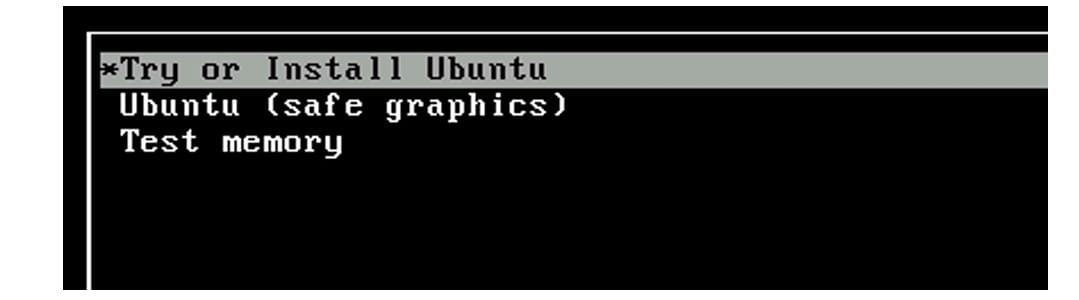
\includegraphics[width=0.5\linewidth]{Imagenes/install}
			\caption{Opciones de inicio/instalación}
			\label{fig:install}
		\end{figure}
		
		En caso de presentar algún tipo de problema con la instalación sobre algún bloqueo de Windows que impida continuar en algún punto con la instalación de de Ubuntu, como lo puede ser el bloqueo de Bitlocker, consultar videos en Youtube o paginas de Internet para solucionarlo, ya que depende mucho del modelo y marca del equipo.
		
		\textcolor{purple}{Solución al bloqueo de Bitlocker:} \url{https://youtu.be/olTCxtPEA_g?si=0crq0c2VNgFkvzFJ}
		
		Una vez seleccionada esta opción iniciara el equipo con el sistema operativo Ubuntu 24.04, en donde aparecerá la pantalla de configuración de idioma entre otras, esas deberán completarse dependiendo del usuario, hasta llegar a esta ventana Figura 10, en donde se seccionaran las siguientes opciones:
		
		\begin{figure}[H]
			\centering
			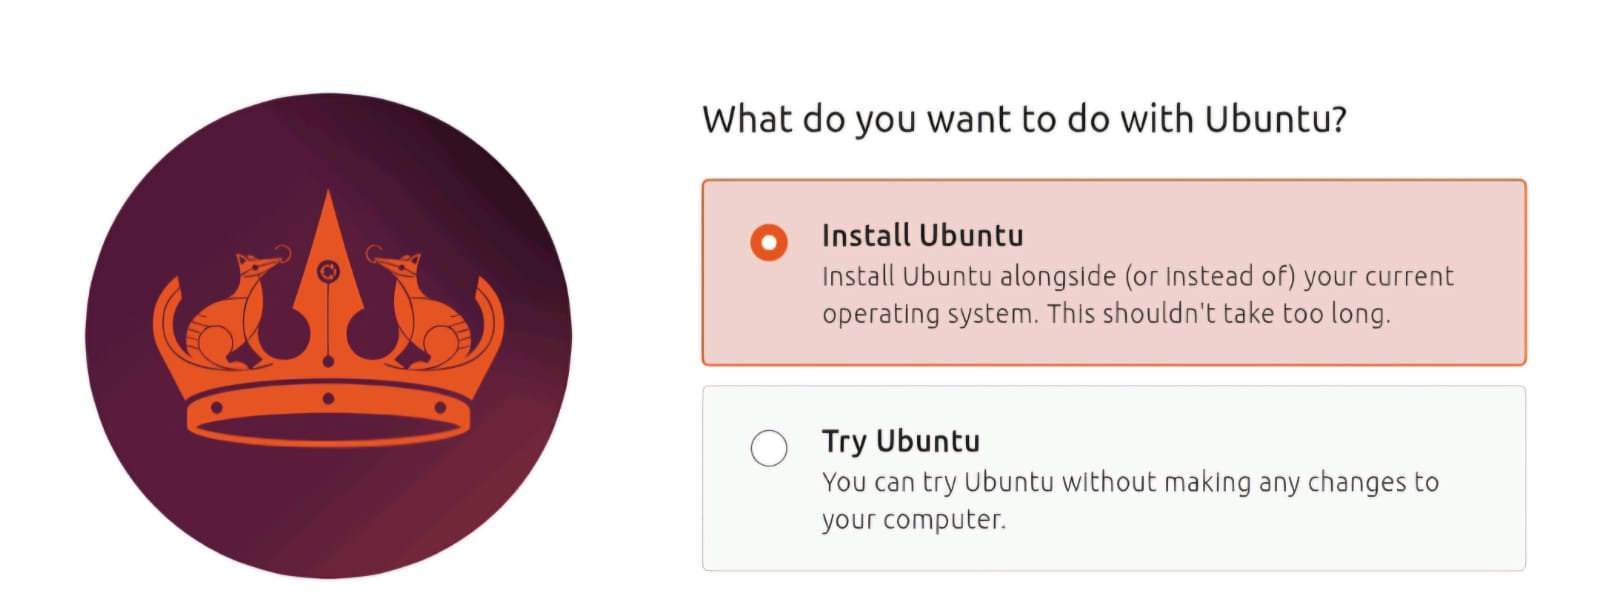
\includegraphics[width=0.5\linewidth]{Imagenes/in1}
			\caption{Instalación}
			\label{fig:in1}
		\end{figure}
		
		\begin{figure}[H]
			\centering
			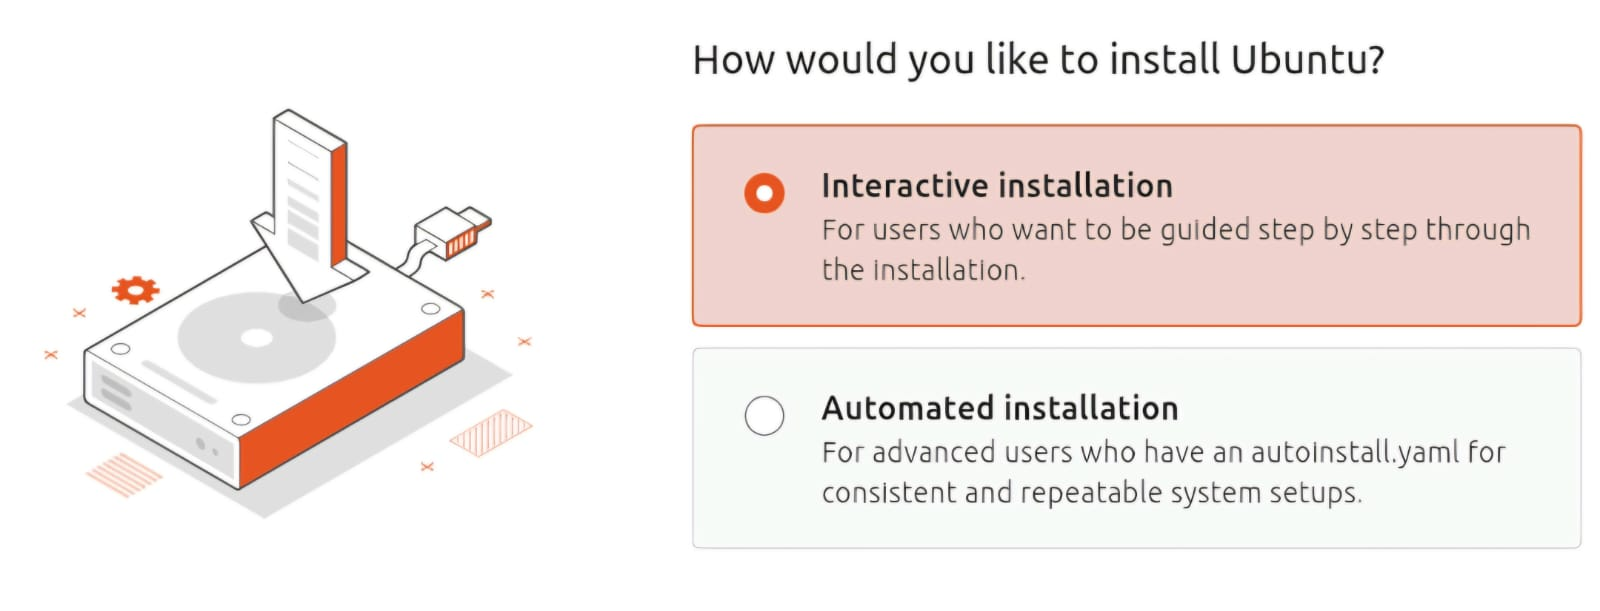
\includegraphics[width=0.5\linewidth]{Imagenes/interactive}
			\caption{Seleccionar Instalación Interactiva}
			\label{fig:interactive}
		\end{figure}
		
		\begin{figure}[H]
			\centering
			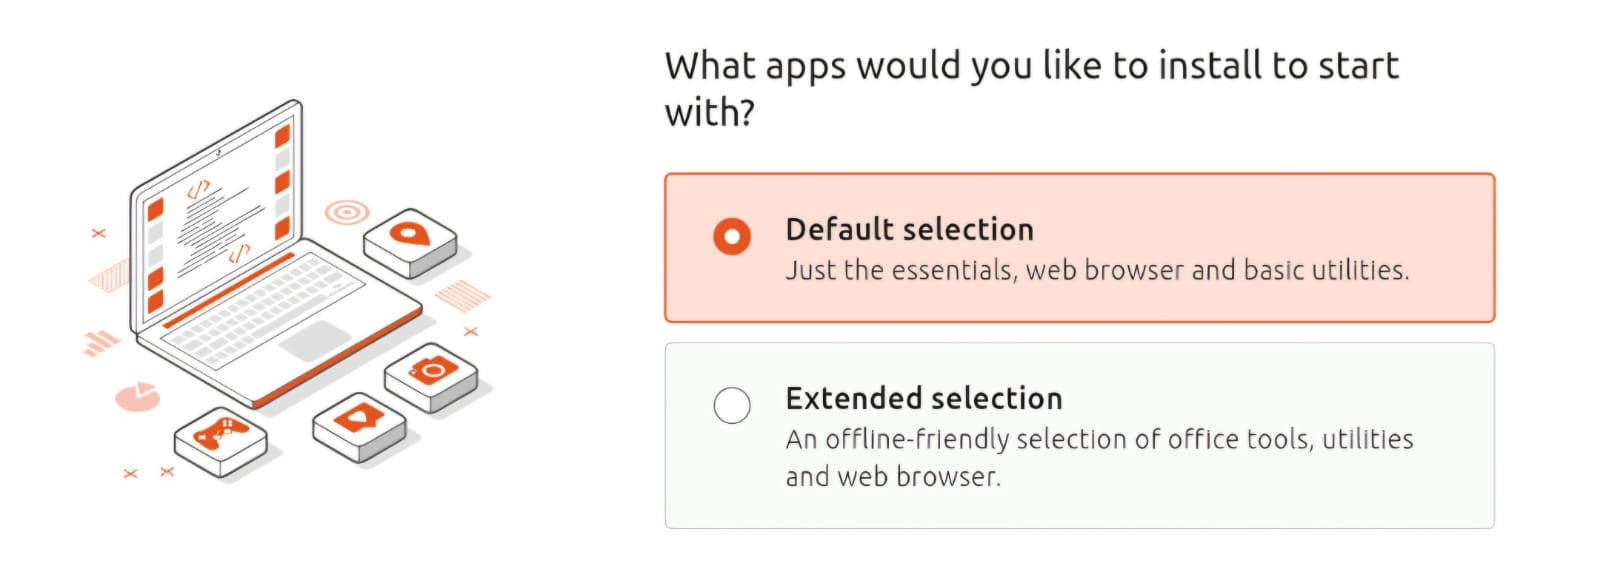
\includegraphics[width=0.5\linewidth]{Imagenes/manual}
			\caption{Seleccionar la opción por defecto}
			\label{fig:manual}
		\end{figure}
		
		\begin{figure}[H]
			\centering
			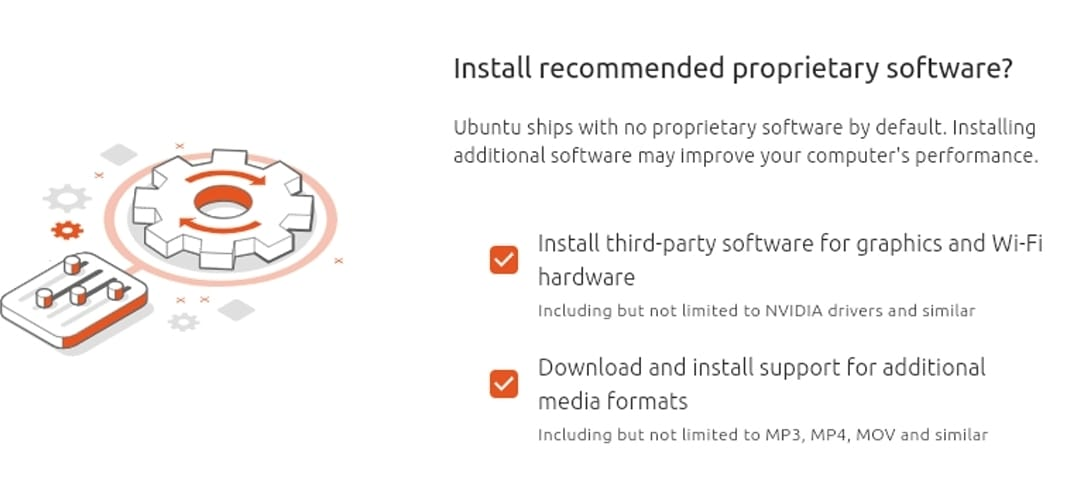
\includegraphics[width=0.5\linewidth]{Imagenes/paqueterias}
			\caption{Seleccionar las dos opciones}
			\label{fig:paqueterias}
		\end{figure}
		
		La opción que se presenta a continuación es \textbf{muy importante y donde se debe de tener más cuidado}, ya que si se llega a hacer mal puede ocasionar perdida de información.
		
		\begin{figure}[H]
			\centering
			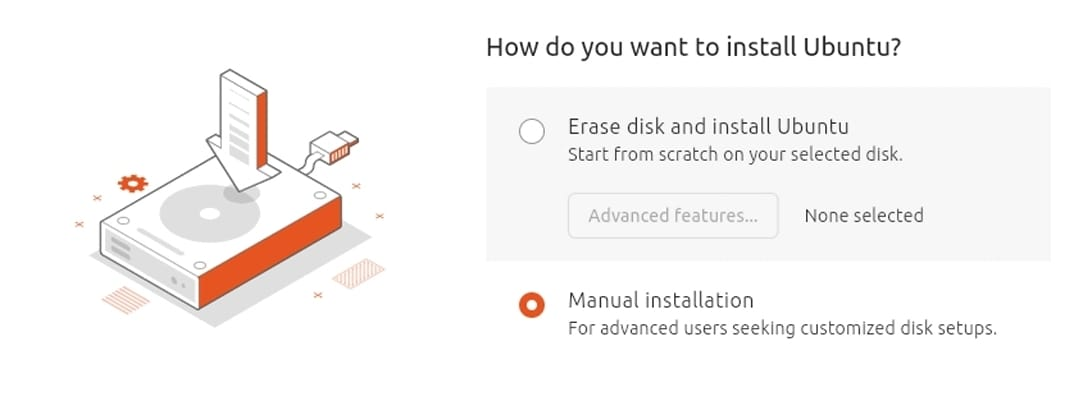
\includegraphics[width=0.5\linewidth]{Imagenes/manual_install}
			\caption{Seleccionar instalación manual}
			\label{fig:manualinstall}
		\end{figure}
		
		Una vez seleccionado la \textbf{instalación manual} aparecerá una ventana con opciones de las distintas particiones que se tienen en el equipo, es aquí donde se tiene que seleccionar la partición con el nombre (\textbf{Free Space o Espacio Libre}) una vez seleccionada, dar click en \textbf{+} en donde se creará un apartado \textbf{swap} como se muestra a continuación y teniendo en cuenta que:
		
		\begin{itemize}
			\item Si tu equipo tiene \textbf{4GB} o menos de RAM se tendrá que poner el doble del tamaño de RAM.
			
			\item Si tu equipo tiene \textbf{8GB} de RAM, se tiene que poner la misma cantidad de tamaño.
			
			\item Si tu equipo tiene \textbf{16GB} o más de RAM se tendrá que poner la mitad del tamaño de RAM.
		\end{itemize}
		
		\begin{figure}[H]
			\centering
			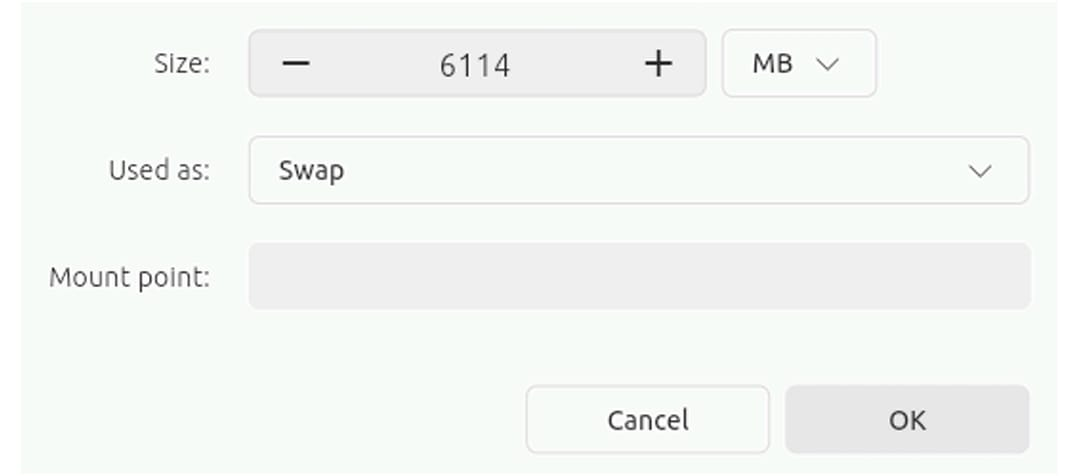
\includegraphics[width=0.5\linewidth]{Imagenes/swap}
			\caption{Creación de Swap}
			\label{fig:swap}
		\end{figure}
		
		Al terminar darle en \textbf{Ok}, y volver a seleccionar la partición de \textbf{Free Space} y seleccionar nuevamente \textbf{+} esta vez el tamaño no se moverá (tendría que aparecer el tamaño restante de los 100GB y lo seleccionado en el swap), esta vez se tendrá que cambiar a estas opciones:
		
		\begin{itemize}
			\item \textbf{Used as:} seleccionar la opción que diga \textbf{Ext4}
			\item \textbf{Mount Point:} seleccionar la raíz: \textbf{$\setminus$}
		\end{itemize}
		
		\begin{figure}[H]
			\centering
			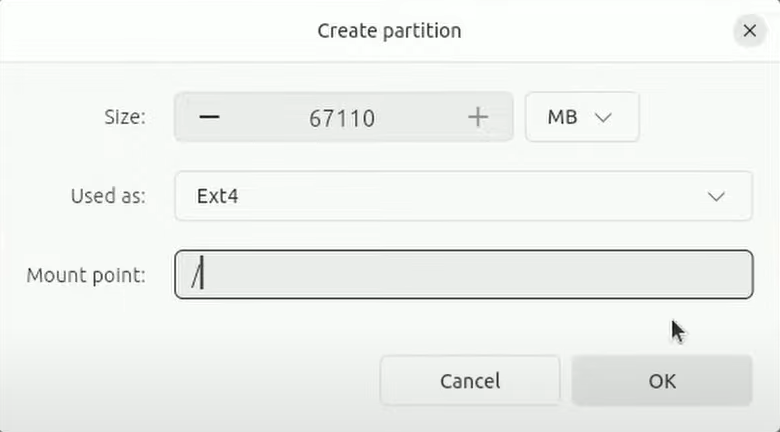
\includegraphics[width=0.4\linewidth]{Imagenes/ext4}
			\caption{Creación de Ext4}
			\label{fig:ext4}
		\end{figure}
		
		
		Una vez terminado tendrán que estar seleccionadas estas dos particiones que se acaban de crear, tanto \textbf{swap} como \textbf{$\setminus$}, se dará en continuar. Lo que hará que empiece con la instalación del S.O. Estas opciones se ven de la siguiente forma o parecidas.\\
		
		\begin{figure}[H]
			\centering
			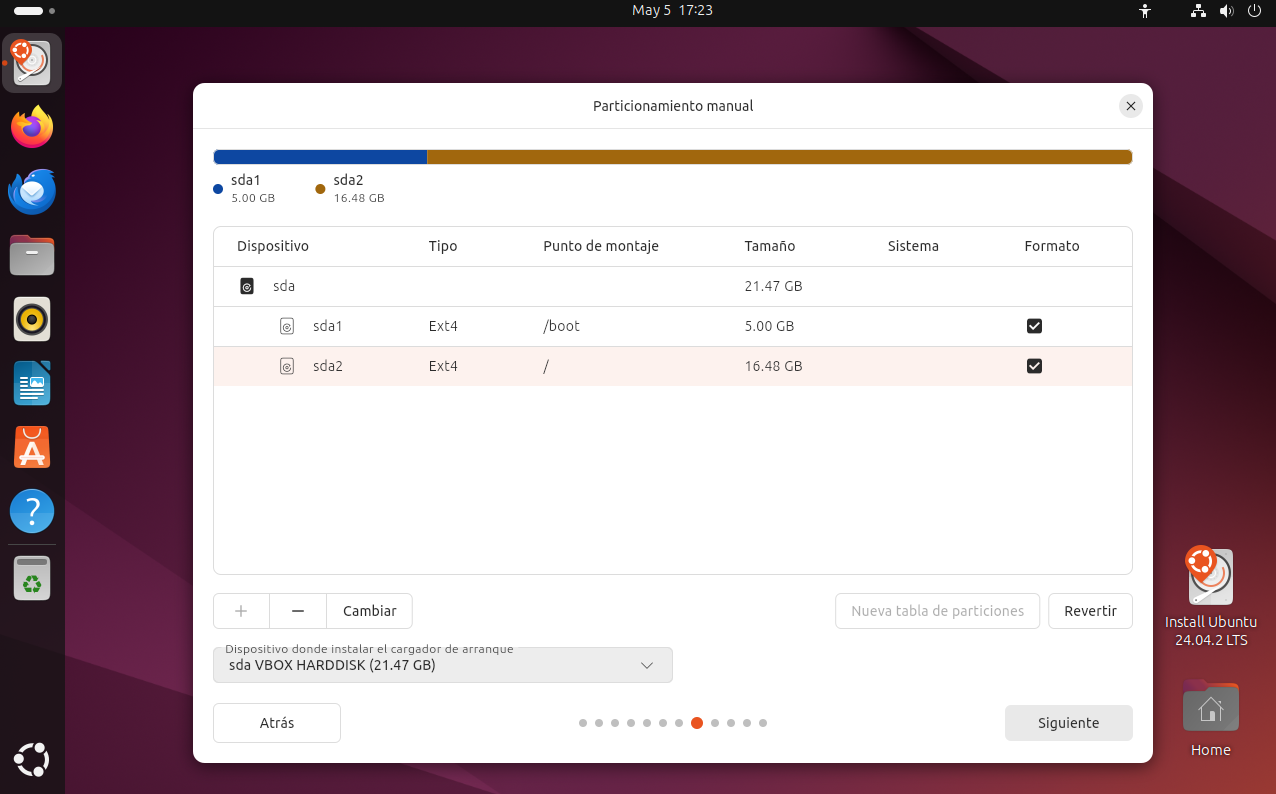
\includegraphics[width=0.5\linewidth]{Imagenes/opciones}
			\caption{Selección de opciones}
			\label{fig:opciones}
		\end{figure}
		
		\textcolor{red}{Nota importante:} Se debe de cuidar que solo se tengan seleccionadas las particiones siguientes: \textbf{Free space}, \textbf{Swap} y \textbf{Ext4 /}. \textcolor{red}{NO SELECCIONAR POR NADA EL WINDOWS BOOT MANAGER.}\\
		
		
		Al acabar la instalación se verá el escritorio como cualquier otro. Posteriormente se abrirá la terminal y se actualizará nuestro entorno, pegando los siguientes comandos en orden.\\
		
		\textbf{sudo apt-get update}\\
		
		\textbf{sudo apt-get upgrade}\\
		
		\textbf{sudo apt-get dist-upgrade}\\
		
		Cada uno de estos comandos hará que nuestro entorno y S.O este actualizado. Una vez concluido se tendrá el nuevo sistema operativo listo para usar.
		
		En caso de tener un equipo MacOS con procesadores Intel, se recomienda el siguiente tutorial para su instalación: \url{https://youtu.be/U3XfZefV0X0?si=z6yM3JG78dG77uc4}
		
	\section{Instalación de Robot Operation System 2 (ROS2)}
	
	Este proyecto utiliza específicamente la versión \textcolor{blue}{ROS2 Jazzy-Jalisco} soportada para Ubuntu 24.04, el cual se instala desde su pagina oficial, siguiendo los comandos indicados.
	
	\textcolor{blue}{\textbf{ROS2 Jazzy-Jalisco: } }\url{https://docs.ros.org/en/jazzy/Installation/Ubuntu-Install-Debs.html}\\
	
	En caso de haber instalado la versión 22.04 de Ubuntu se deberá de instalara ROS2 \textcolor{blue}{Humble Hawksbill}, aunque para la simulación puede presentar algunos errores, y se instala desde el siguiente link:
	
	\textcolor{blue}{\textbf{ROS2 Humble Hawksbill:}} \url{https://docs.ros.org/en/humble/Installation/Ubuntu-Install-Debs.html}\\
	
	\section{Instalación de Webots 2025a}
	
	Para la simulación que se usa en este proyecto, se utiliza un software de simulación llamado Webots, del cual se utiliza la versión 2025a. Para saber más de él consulta la siguiente tarea.
	
	En este link que se proporciona viene el manual de instalación de Webots oficial:
	\url{https://cyberbotics.com/#download}
		
	\end{enumerate}
	
	
	\vspace{0.4cm}
	
\end{document}
